\documentclass{article}
\usepackage[dutch]{babel}
\usepackage{hyperref}
\usepackage{graphicx}


\title{Eindvergadering ML sessie 3}
\author{Team $\exists$uler \and
	\textit{Daan, Marie, Zeineb, Florian, Vincent, Jasper, Lasha, Younes}}
\date{Vrijdag 20 oktober 2023}

\begin{document}
	
\maketitle

\section*{Reflectie}

Dankzij de structuur die we aanbrachten in de KanBan, was het heel duidelijk om overzicht te bewaren over wie waar mee bezig was. Zo was er nooit een moment waarop twee mensen onwetend dezelfde oefening aan het maken waren.

Er zijn nog 7 oefeningen waar we niet aan kunnen beginnen zijn (zoals te zien in figuur \ref{fig:kanban}). De rest van de oefeningen zijn ofwel afgewerkt, ofwel gedeeltelijk afgewerkt. Tegen volgende week is ons objectief om de alle oefeningen af te werken.

\begin{figure}
	\centering
	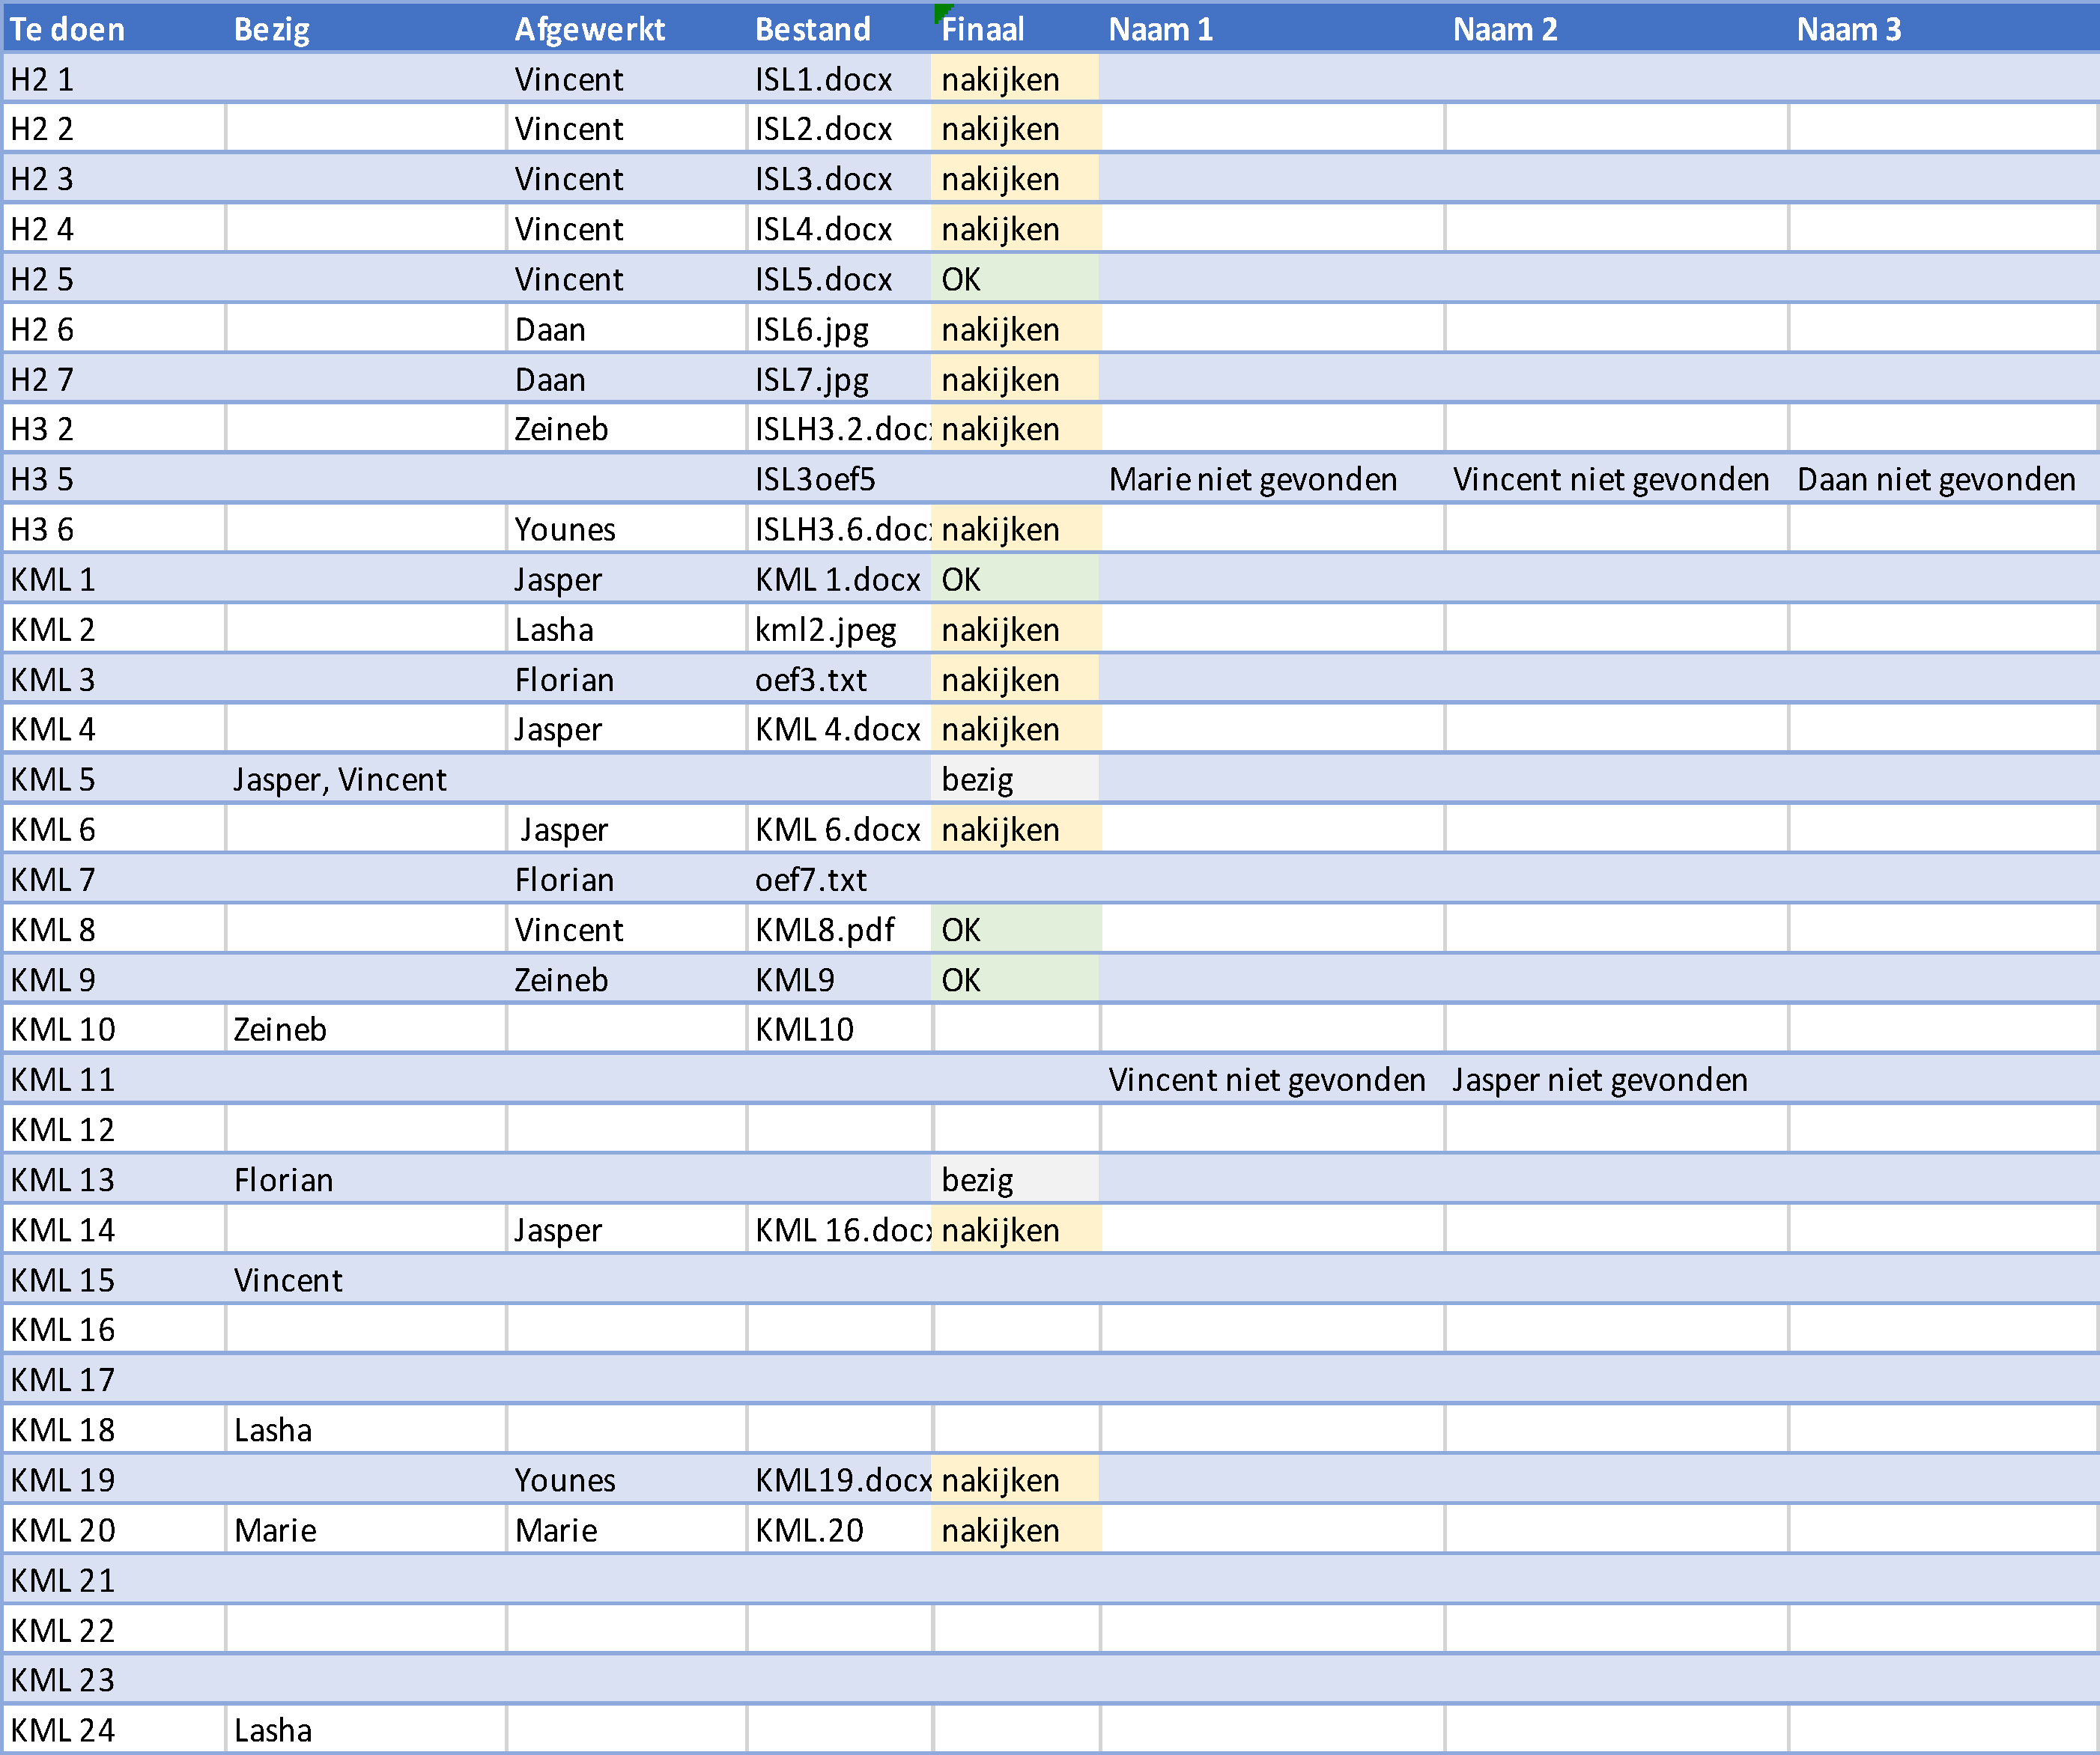
\includegraphics[width=10cm]{kanban}
	\caption{De status van het tabblad \textit{Oefeningen} in de KanBan aan het einde van sessie 3, na twee uur oefeningen maken.}
	\label{fig:kanban}
\end{figure}

\section*{Vooruitblik  \& todo's}

Het was vrij snel duidelijk dat de kernbegrippen over machine learning nog niet bij iedereen gekend zijn. Naar volgende week toe hopen we dus dat iedereen de teksten \textit{ISL} en \textit{MSL} grondig leest en helemaal probeert te begrijpen. Dit zal het afwerken van de oefeningen zeker vergemakkelijken.

Ten slotte hebben we afgesproken dat iedereen zich individueel verdiept in een bepaalde techniek van machine learning tegen volgende week. Dat kan zijn door online research te doen, het boek ISL verder te doorgronden of zelfs video's te kijken op YouTube. Iedereen schrijft over deze technieken een korte en duidelijke tekst en plaatst die vervolgens in de map \textit{ML technieken} op de gedeelde \textit{OneDrive}. Op die manier kan de tekst door de andere groepsleden gelezen worden. Deze technieken zullen we tijdens de startvergadering van sessie 4 dan allemaal bespreken en de beste 3 technieken kiezen. De todo's samengevat:

\begin{itemize}
	\item De teksen \textit{ISL} en \textit{KML} grondig lezen
	\item De oefeningen die nog niet gemaakt zijn op de KanBan afwerken
	\item Elkaars oefeningen die status \textit{nakijken} hebben nakijken en op \textit{OK} zetten
	\item 1 ML techniek bestuderen en een tekst erover in de map \textit{ML technieken} plaatsen
\end{itemize}

\section*{Communicatie}

We hebben ook een \textit{WhatsApp}-groep aangemaakt, waarin we makkelijk met elkaar kunnen communiceren.

\end{document}